%!TEX root = syntheyes15.tex

\section{Our Dynamic Eye-Region Model}

\todo{past tense}

\begin{figure*}
    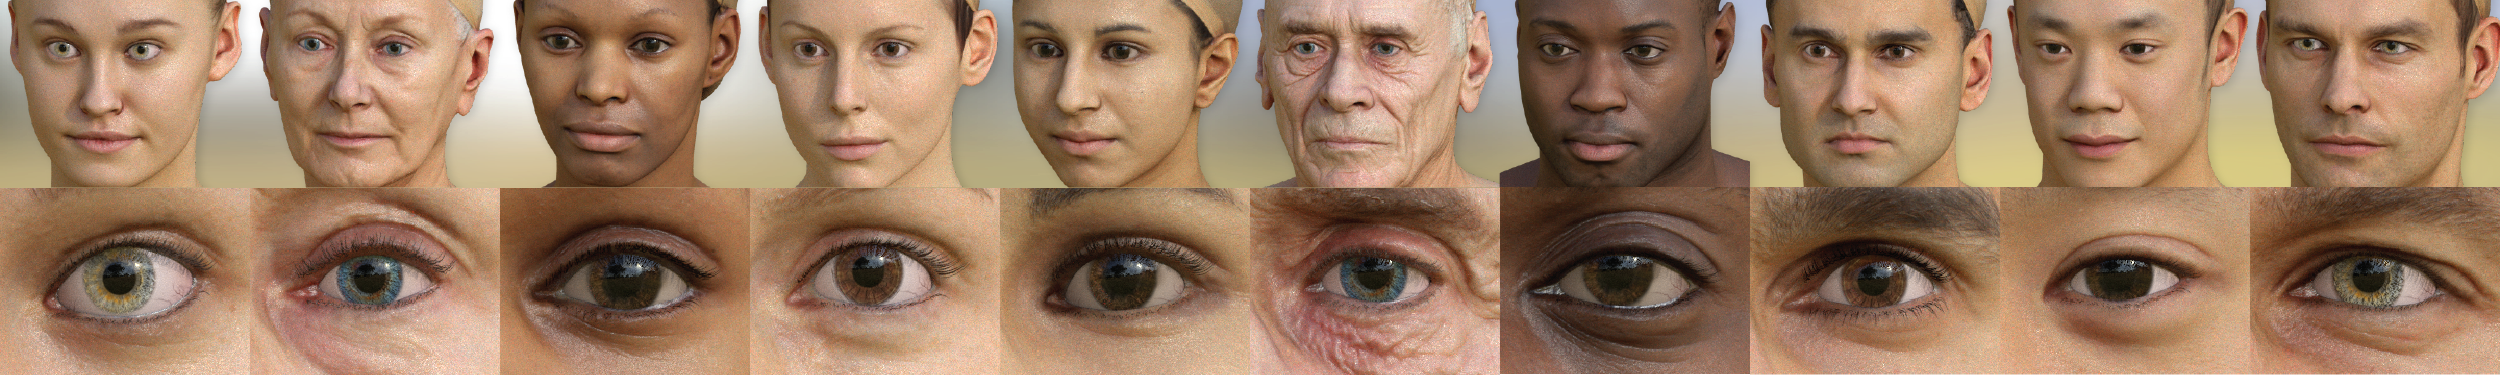
\includegraphics[width=\textwidth]{model_suite}
    \caption{Set of head models and corresponding close-ups of the eye regions used in our method. The set includes 10 different head models of both genders that cover a range of ethnicities and ages.}
    \label{fig:model_suite}
\end{figure*}

In this section we first present our anatomically inspired computer graphics eyeball model, and then explain our novel procedure for preparing a collection of 3D head scans for dynamic photorealistic labelled training data generation.

\subsection{Simplified Eyeball Model}
\label{subsec:eyeball_model}

\begin{figure}
    \centering
    \begin{subfigure}[t]{0.33\columnwidth}
        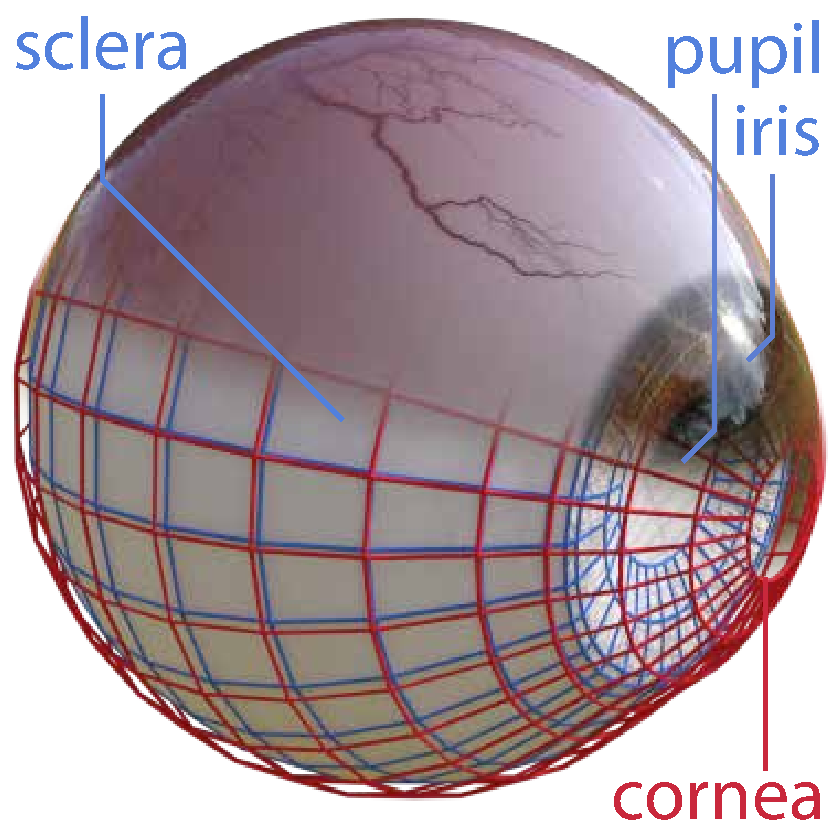
\includegraphics[width=\textwidth]{eye_model}
        \caption{3D eye model}
        \label{fig:3d_eye_model}
    \end{subfigure}%
    \hfill
    \begin{subfigure}[t]{0.65\columnwidth}
        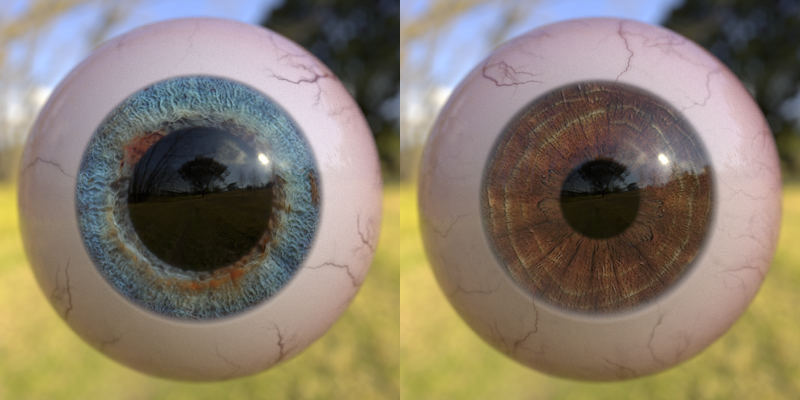
\includegraphics[width=\textwidth]{eye_examples}
        \caption{Pupil dilation and iris color variation}
    \end{subfigure}
    \caption{Our realistic eye model is capable of expressing degrees of variability seen in real life.}
    \label{fig:eye_model}
\end{figure}

% It is important to accurately model reflections and refractions in the eye as they can lead to specular highlights -- these common eye-region image features are often used by eye-tracking algorithms, or can confound approaches that are not robust.

As shown in \autoref{fig:3d_eye_model}, our eye model consists of two parts.
The outer part (red wireframe) approximates the eye's overall shape with two spheres ($r_1\!=\!12\textrm{mm}, r_2\!=\!8\textrm{mm}$ \cite{ruhland2014look}), the latter representing the corneal bulge.
To avoid a discontinuous seam between spheres, their meshes were joined, and the vertices along the seam where smoothed to minimize differences in face-angle.
% \commentA{how joined and smoothed?} Erroll - Maybe needs rewording. Perhaps i'll just put a citation for the smoothing operation? I don't particularly want to describe it
This outer part is transparent, refractive ($n\!=\!1.376$), and partially reflective.
% \commentA{what is transparent?}
The sclera's bumpy surface variations are modelled with smoothed solid noise functions, and applied using a \emph{displacement map} -- a 2D scalar function that shifts a surface in the direction of its normal \cite{lee2000displaced}.
% \commentA{more details on displacement map and noise functions} [Done]
The inner part (blue wireframe) is a flattened sphere with Lambertian material.
The planar end represents the iris and pupil, and the rest represents the sclera -- the white of the eye.
There is a $0.5\textrm{mm}$ gap between the outer and inner parts which accounts for the thickness of the cornea.
\commentE{compare with recent Disney work}

Eyes exhibit variation in both shape (pupillary dilation) and texture (iris color and scleral veins).
To model shape variation we use \emph{blend shapes} -- an animation technique where several different poses are created for the same topological mesh, and then interpolated between\cite{orvalho2012facial}. 
We created blend shapes representing dilated and constricted pupils, as well as large and small irises to account for a small amount ($10\%$) of variation in iris size.
% Maybe try to explain blend shapes better
Blend shapes are localized so can be mixed, so we can easily model an eye with a small pupil, and a large iris.
We vary the texture of the eye by compositing images in three separate layers:
\begin{inparaenum}[\itshape i\upshape)]
\item a \emph{sclera} layer representing the tint of the sclera (white, pink, or yellow);
\item an \emph{iris} layer with four photo-textures of different colored irises (amber, blue, brown, grey); and
\item a \emph{veins} layer which varies between blood-shot and clear.
\end{inparaenum}
We matched the sclera tint to each separate face model but uniformably randomly varied iris color.
% Maybe move to related work?
% Previous research on iris-synthesis \commentE{cite} would have allowed continually different iris textures, but we decided this added complexity would not make a worthwhile improvement in overall appearance variation, especially when rendered at lower resolutions.

\subsection{3D Head Scan Acquisition}
\label{sec:eye_region_geom_prep}

\begin{figure*}
    \centering
    \begin{subfigure}[t]{0.195\textwidth}
        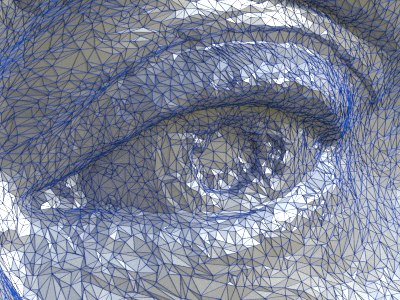
\includegraphics[width=\textwidth]{process_f02_01}
        \caption{Original 3D head scan data: 1.4 million polys}
        \label{fig:process_original_scan}
    \end{subfigure}
    \hfill
    \begin{subfigure}[t]{0.195\textwidth}
        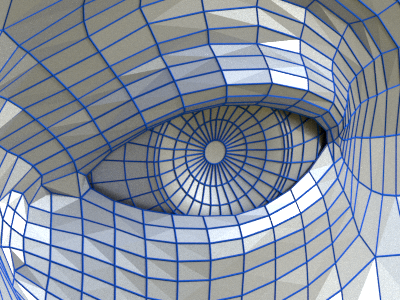
\includegraphics[width=\textwidth]{process_f02_02}
        \caption{Retopologized head model: 9 thousand polys}
        \label{fig:process_retopo}
    \end{subfigure}
    \hfill
    \begin{subfigure}[t]{0.195\textwidth}
        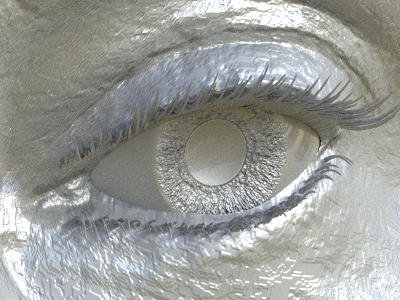
\includegraphics[width=\textwidth]{process_f02_03}
        \caption{Surface detail is stored in displacement maps}
        \label{fig:process_displaced_subdiv}
    \end{subfigure}
    \hfill
    \begin{subfigure}[t]{0.195\textwidth}
        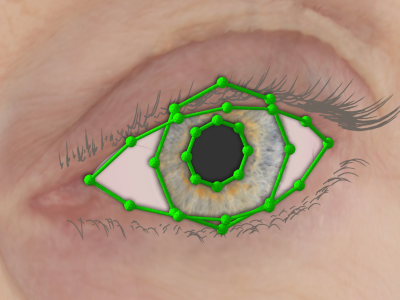
\includegraphics[width=\textwidth]{process_f02_04}
        \caption{3D iris and eyelid landmarks are annotated}
    \end{subfigure}
    \hfill
    \begin{subfigure}[t]{0.195\textwidth}
        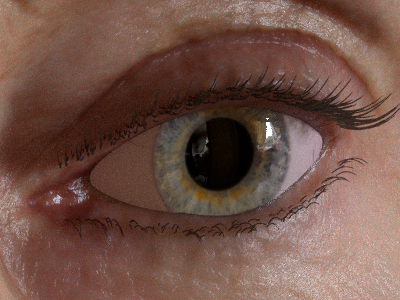
\includegraphics[width=\textwidth]{process_f02_05}
        \caption{The final render}
    \end{subfigure}
    \caption{Model preparation process}
    \label{fig:process}
\end{figure*}

For an eye-region rendering to be realistic, it must also feature realstic nearby face detail. While previous approaches used lifelike artist-created models, for example~\cite{swirski2014rendering}, we instead rely on high quality head scan data captured by a professional photogrammetry studio (10K diffuse color textures, 0.1mm resolution geometry) \cite{Ten24}.
%\commentA{link or even better reference if available}
Nowadays it is possible to cheaply purchase such head scans online\footnote{Ten24 3D Scan Store -- \url{http://www.3dscanstore.com/}} (from $\sim\!\$15$/scan), or use free or commercial photogrammetry software to generate facial geometry models in-house.
A good set of trianing images should exhibit the types of appearance variability seen in real life, therefore our collection of head-models (\autoref{fig:model_suite}) covers both genders with a variety of ethnicities and ages.

\subsection{Eye-Region Geometry Preparation}

As can be seen in \autoref{fig:process_original_scan}, the cornea has been incorrectly reconstructed by the optical scanning process.
This is because transparent surfaces are not directly visible, so cannot be reconstructed in the same way as diffuse surfaces, such as skin.
Recent work used a hybrid reconstruction method to reconstruct the corneal surface separately, but requires additional hardware \cite{berard2014highquality} -- this level of detail was deemed unnecessary for our purposes.
We wanted to render eye-region images representing a wide range of eye-gaze directions, so we needed to be able to pose the eyeball separately from the face geometry.
We therefore removed the scanned eyeball from the mesh using boolean operations, and placed our own eyeball approximation in its place.

While the original head scan geometry is suitable for being rendered as a static model, its topology cannot easily represent dynamic changes in eye-region shape.
Vertical saccades are always accompanied by eyelid motion \cite{liversedge2011oxford}, so we needed to be able to pose the eyelids according to the gaze vector.
When preparing a mesh for facial animation, edge loops should flow along and around the natural contours of facial muscles.
This leads to a more efficient (low-resolution) geometric representation of the face, and more realistic animation as mesh deformation matches that of actual skin tissue and muscles.

% Maybe: \commentE{Reference some other options, e.g automatic methods in research}

We therefore \emph{retopologized} the face geometry into a more optimal form using a commercial semi-automatic system \cite{ZRemesher}.
% Erroll: changed just the sentence below to present tense. As the model still exists, perhaps the tense should be present? Not sure.
As can be seen in \autoref{fig:process_retopo}, edge loops now follow the \emph{Orbicularis Oculi} muscle, allowing for realistic eye-region deformations.
This retopologized low-poly mesh lacks the detail of the original scan (e.g. the crease above the eye), and has visible sharp edges.
We therefore used it as the control mesh for a displaced subdivision surface \cite{lee2000displaced}, with displacement map computed from the scanned geometry.
As can be seen in \autoref{fig:process_displaced_subdiv}, skin surface detail like wrinkles and creases is restored.
Although they are two separate organs, there is normally no visible gap between eyeball and skin.
However, as a consequence of removing the eyeball from the original scan, the retopologized mesh will not necessarily meet the geometry of our eyeball model (see \autoref{fig:process_retopo}).
To compensate for this, the face mesh's eyelid vertices are displaced along their normals to their respective closest positions on the eyeball geometry (see \autoref{fig:process_displaced_subdiv}).
This automatic operation prevents unwanted gaps between the models, even after changes in pose \cite{Shrinkwrap}.

\subsection{Modelling Eyelid Motion}

When someone looks up or down, their eyelids move accordingly \cite{liversedge2011oxford}.
To simulate this we manually created separate blend shapes for upwards-pointing and downwards-pointing eyelids, and interpolate between them based on the global pitch of the eyeball model.
Manually defining blend shapes through vertex manipulation can be a difficult, repetitive, and time-consuming task. Fortunately, only two are required, and they are localized to the eye-region.

\begin{figure}
    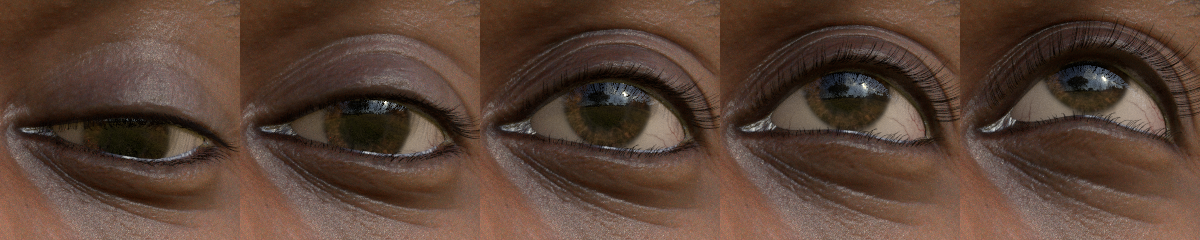
\includegraphics[width=\columnwidth]{eyelid_motion.png}
    \caption{Eyelids are posed using blend shapes linked to the gaze vector. Note how we use wrinkle-maps to simulate the folding of the skin above and below the eye.}
\end{figure}

\subsection{Modelling of Eyelashes}

Eyelashes are short curved hairs that grow from the outer edges of the eyelids.
These can occlude parts of the eye and affect eye tracking algorithms, so are simulated as part of our comprehensive model.
We followed the approach of \citet{swirski2014rendering}, and model eyelashes using directed hair particle effects.
The hair particles were generated from a control surface manually placed below the eyelids.
To make them curl, eyelash particles experience a slight amount of gravity during growth (negative gravity for the upper eyelash).

\subsection{Eye-Region Landmark Annotation}

As shown in \autoref{fig:process_ldmks}, each 3D eye-region was annotated in 3D with $28$ landmarks, corresponding to the eye corners ($2$), eyelids ($5\!+\!5$), iris boundary ($8$), and pupil boundary ($8$).
The iris and pupil landmarks were defined as a subset of the eyeball geometry vertices, so deform automatically with changes in pupil and iris size.
The eyelid and eye corner landmarks were manually labelled with a separate mesh that follows the seam where eyeball geometry meets skin geometry.
This mesh is assigned shape keys so deforms automatically during eyelid motion.
%
% So instead of having humans ambiguously label eye-region anatomy, we carefully manually annotate each eye-region once, ensuring higher-quality labels.
% Maybe put the sentence below in later
Whenever an image is rendered, the 2D image-space coordinates of these 3D landmarks are calculated using the camera projection matrix and saved.